% Options for packages loaded elsewhere
\PassOptionsToPackage{unicode}{hyperref}
\PassOptionsToPackage{hyphens}{url}
%
\documentclass[
]{article}
\usepackage{amsmath,amssymb}
\usepackage{lmodern}
\usepackage{ifxetex,ifluatex}
\ifnum 0\ifxetex 1\fi\ifluatex 1\fi=0 % if pdftex
  \usepackage[T1]{fontenc}
  \usepackage[utf8]{inputenc}
  \usepackage{textcomp} % provide euro and other symbols
\else % if luatex or xetex
  \usepackage{unicode-math}
  \defaultfontfeatures{Scale=MatchLowercase}
  \defaultfontfeatures[\rmfamily]{Ligatures=TeX,Scale=1}
\fi
% Use upquote if available, for straight quotes in verbatim environments
\IfFileExists{upquote.sty}{\usepackage{upquote}}{}
\IfFileExists{microtype.sty}{% use microtype if available
  \usepackage[]{microtype}
  \UseMicrotypeSet[protrusion]{basicmath} % disable protrusion for tt fonts
}{}
\makeatletter
\@ifundefined{KOMAClassName}{% if non-KOMA class
  \IfFileExists{parskip.sty}{%
    \usepackage{parskip}
  }{% else
    \setlength{\parindent}{0pt}
    \setlength{\parskip}{6pt plus 2pt minus 1pt}}
}{% if KOMA class
  \KOMAoptions{parskip=half}}
\makeatother
\usepackage{xcolor}
\IfFileExists{xurl.sty}{\usepackage{xurl}}{} % add URL line breaks if available
\IfFileExists{bookmark.sty}{\usepackage{bookmark}}{\usepackage{hyperref}}
\hypersetup{
  pdftitle={morales-exam3},
  pdfauthor={Laura Morales},
  hidelinks,
  pdfcreator={LaTeX via pandoc}}
\urlstyle{same} % disable monospaced font for URLs
\usepackage[margin=1in]{geometry}
\usepackage{color}
\usepackage{fancyvrb}
\newcommand{\VerbBar}{|}
\newcommand{\VERB}{\Verb[commandchars=\\\{\}]}
\DefineVerbatimEnvironment{Highlighting}{Verbatim}{commandchars=\\\{\}}
% Add ',fontsize=\small' for more characters per line
\usepackage{framed}
\definecolor{shadecolor}{RGB}{248,248,248}
\newenvironment{Shaded}{\begin{snugshade}}{\end{snugshade}}
\newcommand{\AlertTok}[1]{\textcolor[rgb]{0.94,0.16,0.16}{#1}}
\newcommand{\AnnotationTok}[1]{\textcolor[rgb]{0.56,0.35,0.01}{\textbf{\textit{#1}}}}
\newcommand{\AttributeTok}[1]{\textcolor[rgb]{0.77,0.63,0.00}{#1}}
\newcommand{\BaseNTok}[1]{\textcolor[rgb]{0.00,0.00,0.81}{#1}}
\newcommand{\BuiltInTok}[1]{#1}
\newcommand{\CharTok}[1]{\textcolor[rgb]{0.31,0.60,0.02}{#1}}
\newcommand{\CommentTok}[1]{\textcolor[rgb]{0.56,0.35,0.01}{\textit{#1}}}
\newcommand{\CommentVarTok}[1]{\textcolor[rgb]{0.56,0.35,0.01}{\textbf{\textit{#1}}}}
\newcommand{\ConstantTok}[1]{\textcolor[rgb]{0.00,0.00,0.00}{#1}}
\newcommand{\ControlFlowTok}[1]{\textcolor[rgb]{0.13,0.29,0.53}{\textbf{#1}}}
\newcommand{\DataTypeTok}[1]{\textcolor[rgb]{0.13,0.29,0.53}{#1}}
\newcommand{\DecValTok}[1]{\textcolor[rgb]{0.00,0.00,0.81}{#1}}
\newcommand{\DocumentationTok}[1]{\textcolor[rgb]{0.56,0.35,0.01}{\textbf{\textit{#1}}}}
\newcommand{\ErrorTok}[1]{\textcolor[rgb]{0.64,0.00,0.00}{\textbf{#1}}}
\newcommand{\ExtensionTok}[1]{#1}
\newcommand{\FloatTok}[1]{\textcolor[rgb]{0.00,0.00,0.81}{#1}}
\newcommand{\FunctionTok}[1]{\textcolor[rgb]{0.00,0.00,0.00}{#1}}
\newcommand{\ImportTok}[1]{#1}
\newcommand{\InformationTok}[1]{\textcolor[rgb]{0.56,0.35,0.01}{\textbf{\textit{#1}}}}
\newcommand{\KeywordTok}[1]{\textcolor[rgb]{0.13,0.29,0.53}{\textbf{#1}}}
\newcommand{\NormalTok}[1]{#1}
\newcommand{\OperatorTok}[1]{\textcolor[rgb]{0.81,0.36,0.00}{\textbf{#1}}}
\newcommand{\OtherTok}[1]{\textcolor[rgb]{0.56,0.35,0.01}{#1}}
\newcommand{\PreprocessorTok}[1]{\textcolor[rgb]{0.56,0.35,0.01}{\textit{#1}}}
\newcommand{\RegionMarkerTok}[1]{#1}
\newcommand{\SpecialCharTok}[1]{\textcolor[rgb]{0.00,0.00,0.00}{#1}}
\newcommand{\SpecialStringTok}[1]{\textcolor[rgb]{0.31,0.60,0.02}{#1}}
\newcommand{\StringTok}[1]{\textcolor[rgb]{0.31,0.60,0.02}{#1}}
\newcommand{\VariableTok}[1]{\textcolor[rgb]{0.00,0.00,0.00}{#1}}
\newcommand{\VerbatimStringTok}[1]{\textcolor[rgb]{0.31,0.60,0.02}{#1}}
\newcommand{\WarningTok}[1]{\textcolor[rgb]{0.56,0.35,0.01}{\textbf{\textit{#1}}}}
\usepackage{graphicx}
\makeatletter
\def\maxwidth{\ifdim\Gin@nat@width>\linewidth\linewidth\else\Gin@nat@width\fi}
\def\maxheight{\ifdim\Gin@nat@height>\textheight\textheight\else\Gin@nat@height\fi}
\makeatother
% Scale images if necessary, so that they will not overflow the page
% margins by default, and it is still possible to overwrite the defaults
% using explicit options in \includegraphics[width, height, ...]{}
\setkeys{Gin}{width=\maxwidth,height=\maxheight,keepaspectratio}
% Set default figure placement to htbp
\makeatletter
\def\fps@figure{htbp}
\makeatother
\setlength{\emergencystretch}{3em} % prevent overfull lines
\providecommand{\tightlist}{%
  \setlength{\itemsep}{0pt}\setlength{\parskip}{0pt}}
\setcounter{secnumdepth}{-\maxdimen} % remove section numbering
\ifluatex
  \usepackage{selnolig}  % disable illegal ligatures
\fi

\title{morales-exam3}
\author{Laura Morales}
\date{7/8/2021}

\begin{document}
\maketitle

\hypertarget{question-1-clear-environment}{%
\subsection{Question 1: Clear
environment}\label{question-1-clear-environment}}

\begin{Shaded}
\begin{Highlighting}[]
\CommentTok{\#clear environment }
\FunctionTok{rm}\NormalTok{(}\AttributeTok{list =} \FunctionTok{ls}\NormalTok{(}\AttributeTok{all=}\ConstantTok{TRUE}\NormalTok{))}
\end{Highlighting}
\end{Shaded}

\hypertarget{question-2-load-wdi-package-and-female-labor-force-participation}{%
\subsection{Question 2: load WDI package and female labor force
participation}\label{question-2-load-wdi-package-and-female-labor-force-participation}}

\begin{Shaded}
\begin{Highlighting}[]
\CommentTok{\#load all necessary libraries }
\FunctionTok{library}\NormalTok{(rio)}
\FunctionTok{library}\NormalTok{(tidyverse)}
\end{Highlighting}
\end{Shaded}

\begin{verbatim}
## -- Attaching packages --------------------------------------- tidyverse 1.3.1 --
\end{verbatim}

\begin{verbatim}
## v ggplot2 3.3.5     v purrr   0.3.4
## v tibble  3.1.2     v dplyr   1.0.7
## v tidyr   1.1.3     v stringr 1.4.0
## v readr   1.4.0     v forcats 0.5.1
\end{verbatim}

\begin{verbatim}
## -- Conflicts ------------------------------------------ tidyverse_conflicts() --
## x dplyr::filter() masks stats::filter()
## x dplyr::lag()    masks stats::lag()
\end{verbatim}

\begin{Shaded}
\begin{Highlighting}[]
\FunctionTok{library}\NormalTok{(googlesheets4)}
\FunctionTok{library}\NormalTok{(labelled)}
\FunctionTok{library}\NormalTok{(data.table)}
\end{Highlighting}
\end{Shaded}

\begin{verbatim}
## 
## Attaching package: 'data.table'
\end{verbatim}

\begin{verbatim}
## The following objects are masked from 'package:dplyr':
## 
##     between, first, last
\end{verbatim}

\begin{verbatim}
## The following object is masked from 'package:purrr':
## 
##     transpose
\end{verbatim}

\begin{Shaded}
\begin{Highlighting}[]
\FunctionTok{library}\NormalTok{(varhandle)}
\FunctionTok{library}\NormalTok{(ggrepel)}
\FunctionTok{library}\NormalTok{(geosphere)}
\FunctionTok{library}\NormalTok{(rgeos)}
\end{Highlighting}
\end{Shaded}

\begin{verbatim}
## Loading required package: sp
\end{verbatim}

\begin{verbatim}
## rgeos version: 0.5-5, (SVN revision 640)
##  GEOS runtime version: 3.8.1-CAPI-1.13.3 
##  Linking to sp version: 1.4-2 
##  Polygon checking: TRUE
\end{verbatim}

\begin{Shaded}
\begin{Highlighting}[]
\FunctionTok{library}\NormalTok{(viridis)}
\end{Highlighting}
\end{Shaded}

\begin{verbatim}
## Loading required package: viridisLite
\end{verbatim}

\begin{Shaded}
\begin{Highlighting}[]
\FunctionTok{library}\NormalTok{(mapview)}
\FunctionTok{library}\NormalTok{(rnaturalearth)}
\FunctionTok{library}\NormalTok{(rnaturalearthdata)}
\FunctionTok{library}\NormalTok{(devtools)}
\end{Highlighting}
\end{Shaded}

\begin{verbatim}
## Loading required package: usethis
\end{verbatim}

\begin{Shaded}
\begin{Highlighting}[]
\NormalTok{devtools}\SpecialCharTok{::}\FunctionTok{install\_github}\NormalTok{(}\StringTok{"ropensci/rnaturalearthhires"}\NormalTok{)}
\end{Highlighting}
\end{Shaded}

\begin{verbatim}
## Skipping install of 'rnaturalearthhires' from a github remote, the SHA1 (2ed7a937) has not changed since last install.
##   Use `force = TRUE` to force installation
\end{verbatim}

\begin{Shaded}
\begin{Highlighting}[]
\FunctionTok{library}\NormalTok{(rnaturalearthhires)}
\FunctionTok{library}\NormalTok{(raster)}
\end{Highlighting}
\end{Shaded}

\begin{verbatim}
## 
## Attaching package: 'raster'
\end{verbatim}

\begin{verbatim}
## The following object is masked from 'package:data.table':
## 
##     shift
\end{verbatim}

\begin{verbatim}
## The following object is masked from 'package:dplyr':
## 
##     select
\end{verbatim}

\begin{verbatim}
## The following object is masked from 'package:tidyr':
## 
##     extract
\end{verbatim}

\begin{Shaded}
\begin{Highlighting}[]
\FunctionTok{library}\NormalTok{(sp)}
\FunctionTok{library}\NormalTok{(sf)}
\end{Highlighting}
\end{Shaded}

\begin{verbatim}
## Linking to GEOS 3.8.1, GDAL 3.2.1, PROJ 7.2.1
\end{verbatim}

\begin{Shaded}
\begin{Highlighting}[]
\NormalTok{devtools}\SpecialCharTok{::}\FunctionTok{install\_github}\NormalTok{(}\StringTok{"yutannihilation/ggsflabel"}\NormalTok{)}
\end{Highlighting}
\end{Shaded}

\begin{verbatim}
## Skipping install of 'ggsflabel' from a github remote, the SHA1 (a489481b) has not changed since last install.
##   Use `force = TRUE` to force installation
\end{verbatim}

\begin{Shaded}
\begin{Highlighting}[]
\FunctionTok{library}\NormalTok{(ggsflabel)}
\end{Highlighting}
\end{Shaded}

\begin{verbatim}
## 
## Attaching package: 'ggsflabel'
\end{verbatim}

\begin{verbatim}
## The following objects are masked from 'package:ggplot2':
## 
##     geom_sf_label, geom_sf_text, StatSfCoordinates
\end{verbatim}

\begin{Shaded}
\begin{Highlighting}[]
\FunctionTok{library}\NormalTok{(Imap)}
\end{Highlighting}
\end{Shaded}

\begin{verbatim}
## 
## Attaching package: 'Imap'
\end{verbatim}

\begin{verbatim}
## The following object is masked from 'package:purrr':
## 
##     imap
\end{verbatim}

\begin{Shaded}
\begin{Highlighting}[]
\FunctionTok{library}\NormalTok{(ggplot2)}
\FunctionTok{library}\NormalTok{(dplyr)}
\FunctionTok{library}\NormalTok{(WDI)}
\FunctionTok{library}\NormalTok{(countrycode)}
\CommentTok{\#load the WDi data}
\NormalTok{female\_lfp }\OtherTok{=} \FunctionTok{WDI}\NormalTok{(}\AttributeTok{country =} \StringTok{"all"}\NormalTok{, }\AttributeTok{indicator =} \FunctionTok{c}\NormalTok{(}\StringTok{"SL.TLF.CACT.FE.ZS"}\NormalTok{), }\AttributeTok{start =} \DecValTok{2010}\NormalTok{, }\AttributeTok{end =} \DecValTok{2015}\NormalTok{, }\AttributeTok{cache =} \ConstantTok{NULL}\NormalTok{)}
\end{Highlighting}
\end{Shaded}

\hypertarget{question-3-rename-variable}{%
\subsection{Question 3: rename
variable}\label{question-3-rename-variable}}

\begin{Shaded}
\begin{Highlighting}[]
\CommentTok{\#rename the variable}
\NormalTok{female\_lfp }\OtherTok{\textless{}{-}} \FunctionTok{rename}\NormalTok{(female\_lfp, }\StringTok{"flfp"}\OtherTok{=}\StringTok{"SL.TLF.CACT.FE.ZS"}\NormalTok{)}
\end{Highlighting}
\end{Shaded}

\hypertarget{question-4-collapse-female_lfpby-the-mean-value-forflfp}{%
\subsection{Question 4: collapse female\_lfpby the mean value
forflfp}\label{question-4-collapse-female_lfpby-the-mean-value-forflfp}}

\begin{Shaded}
\begin{Highlighting}[]
\CommentTok{\#collapse female\_lfpby the mean value forflfp }
\NormalTok{collapsed\_flfp}\OtherTok{=}\NormalTok{ female\_lfp }\SpecialCharTok{\%\textgreater{}\%} \FunctionTok{group\_by}\NormalTok{(country, iso2c) }\SpecialCharTok{\%\textgreater{}\%} \FunctionTok{summarise}\NormalTok{(}\AttributeTok{flfp =} \FunctionTok{mean}\NormalTok{(flfp), }\AttributeTok{na.rm=}\ConstantTok{TRUE}\NormalTok{) }
\end{Highlighting}
\end{Shaded}

\begin{verbatim}
## `summarise()` has grouped output by 'country'. You can override using the `.groups` argument.
\end{verbatim}

\hypertarget{question-5-countries-which-have-an-average-female-force-participation-rates-less-than-15}\label{question-5-countries-which-have-an-average-female-force-participation-rates-less-than-15}}

\begin{Shaded}
\begin{Highlighting}[]
\CommentTok{\#filter those over 15\%}
\NormalTok{less\_15 }\OtherTok{\textless{}{-}} \FunctionTok{filter}\NormalTok{(collapsed\_flfp, flfp }\SpecialCharTok{\textless{}} \DecValTok{15}\NormalTok{ )}
\end{Highlighting}
\end{Shaded}

\hypertarget{question-6-map-of-the-world-of-usingcollapsed_flfp-using-the-viridis-colorschem}{%
\subsection{Question 6: Map of the world of usingcollapsed\_flfp, using
the viridis
colorschem}\label{question-6-map-of-the-world-of-usingcollapsed_flfp-using-the-viridis-colorschem}}

\begin{Shaded}
\begin{Highlighting}[]
\CommentTok{\#load world borders}
\NormalTok{world\_borders }\OtherTok{\textless{}{-}} \FunctionTok{st\_read}\NormalTok{(}\StringTok{"/Users/lauram./Documents/Gov 355M Data Sci for Soc/Mods/Mod 11/world border shape files/World\_Borders.shp"}\NormalTok{)}
\end{Highlighting}
\end{Shaded}

\begin{verbatim}
## Reading layer `World_Borders' from data source 
##   `/Users/lauram./Documents/Gov 355M Data Sci for Soc/Mods/Mod 11/world border shape files/World_Borders.shp' 
##   using driver `ESRI Shapefile'
## Simple feature collection with 246 features and 11 fields
## Geometry type: MULTIPOLYGON
## Dimension:     XY
## Bounding box:  xmin: -180 ymin: -90 xmax: 180 ymax: 83.6236
## Geodetic CRS:  WGS 84
\end{verbatim}

\begin{Shaded}
\begin{Highlighting}[]
\CommentTok{\#transform to WGS84 projection}
\NormalTok{borders }\OtherTok{=} \FunctionTok{st\_transform}\NormalTok{(world\_borders, }\StringTok{"+proj=latlong +ellps=WGS84 +datum=WGS84"}\NormalTok{)}
\FunctionTok{rm}\NormalTok{(world\_borders)}
\CommentTok{\#merege the codes and coordinates}
\NormalTok{collapsed\_flfp}\SpecialCharTok{$}\NormalTok{ISO3}\OtherTok{=} \FunctionTok{countrycode}\NormalTok{(}\AttributeTok{sourcevar =}\NormalTok{ collapsed\_flfp}\SpecialCharTok{$}\NormalTok{country, }\AttributeTok{origin =} \StringTok{"country.name"}\NormalTok{, }\AttributeTok{destination=}\StringTok{"iso3c"}\NormalTok{, }\AttributeTok{warn=}\ConstantTok{TRUE}\NormalTok{)}
\end{Highlighting}
\end{Shaded}

\begin{verbatim}
## Warning in countrycode(sourcevar = collapsed_flfp$country, origin = "country.name", : Some values were not matched unambiguously: Africa Eastern and Southern, Africa Western and Central, Arab World, Caribbean small states, Central Europe and the Baltics, Channel Islands, Early-demographic dividend, East Asia & Pacific, East Asia & Pacific (excluding high income), East Asia & Pacific (IDA & IBRD countries), Euro area, Europe & Central Asia, Europe & Central Asia (excluding high income), Europe & Central Asia (IDA & IBRD countries), European Union, Fragile and conflict affected situations, Heavily indebted poor countries (HIPC), High income, IBRD only, IDA & IBRD total, IDA blend, IDA only, IDA total, Kosovo, Late-demographic dividend, Latin America & Caribbean, Latin America & Caribbean (excluding high income), Latin America & the Caribbean (IDA & IBRD countries), Least developed countries: UN classification, Low & middle income, Low income, Lower middle income, Middle East & North Africa, Middle East & North Africa (excluding high income), Middle East & North Africa (IDA & IBRD countries), Middle income, North America, Not classified, OECD members, Other small states, Pacific island small states, Post-demographic dividend, Pre-demographic dividend, Small states, South Asia, South Asia (IDA & IBRD), Sub-Saharan Africa, Sub-Saharan Africa (excluding high income), Sub-Saharan Africa (IDA & IBRD countries), Upper middle income, World
\end{verbatim}

\begin{Shaded}
\begin{Highlighting}[]
\NormalTok{collapsed\_flfp\_small }\OtherTok{=} \FunctionTok{na.omit}\NormalTok{(collapsed\_flfp, }\FunctionTok{select}\NormalTok{(}\StringTok{"country"}\NormalTok{, }\StringTok{"flfp"}\NormalTok{, }\StringTok{"ISO3"}\NormalTok{))}
\NormalTok{merged\_data}\OtherTok{=} \FunctionTok{left\_join}\NormalTok{(borders, collapsed\_flfp\_small, }\AttributeTok{by=}\StringTok{"ISO3"}\NormalTok{)}
\CommentTok{\#create the map}
\NormalTok{flfp\_map}\OtherTok{=} \FunctionTok{ggplot}\NormalTok{()}\SpecialCharTok{+}
  \FunctionTok{geom\_sf}\NormalTok{(}\AttributeTok{data=}\NormalTok{borders)}\SpecialCharTok{+}
  \FunctionTok{geom\_sf}\NormalTok{(}\AttributeTok{data=}\NormalTok{merged\_data, }\FunctionTok{aes}\NormalTok{(}\AttributeTok{fill=}\NormalTok{flfp))}\SpecialCharTok{+}
  \FunctionTok{scale\_fill\_viridis}\NormalTok{(}\AttributeTok{option=}\StringTok{"viridis"}\NormalTok{)}\SpecialCharTok{+}
  \FunctionTok{ggtitle}\NormalTok{(}\StringTok{"World Wide Female Labor Forced Participation (percent), 2010{-}2015"}\NormalTok{)}\SpecialCharTok{+}
  \FunctionTok{theme}\NormalTok{(}\AttributeTok{plot.title=} \FunctionTok{element\_text}\NormalTok{(}\AttributeTok{hjust =} \FloatTok{0.5}\NormalTok{))}\SpecialCharTok{+}
  \FunctionTok{theme\_void}\NormalTok{()}
\FunctionTok{print}\NormalTok{(flfp\_map)}
\end{Highlighting}
\end{Shaded}

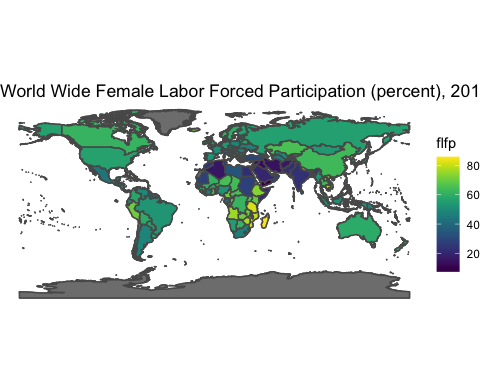
\includegraphics{exam-3_files/figure-latex/unnamed-chunk-6-1.pdf} \#\#
Question 7: Based on the map, which area of the world has, perhaps
surprisingly, a cluster of yellow-colored average female labor force
participation rate states, indicating the highest onthe scale?

I thought it was surprising that south easter africa has a very high
female labor participation.

\hypertarget{question-8-use-r-to-show-the-same-cluster-of-states-referenced-in-the-previous-question.}{%
\subsection{Question 8: Use R to show the same cluster of states
referenced in the previous
question.}\label{question-8-use-r-to-show-the-same-cluster-of-states-referenced-in-the-previous-question.}}

\begin{Shaded}
\begin{Highlighting}[]
\CommentTok{\#subset data to only referenced countries}
\NormalTok{sa\_fl }\OtherTok{\textless{}{-}} \FunctionTok{subset}\NormalTok{(merged\_data, country}\SpecialCharTok{==}\StringTok{"Madagascar"}\SpecialCharTok{|}\NormalTok{ country}\SpecialCharTok{==}\StringTok{"Mozambique"}\SpecialCharTok{|}\NormalTok{ country}\SpecialCharTok{==}\StringTok{"Tanzania"}\NormalTok{)}
\NormalTok{sa\_fl\_map }\OtherTok{\textless{}{-}} \FunctionTok{subset}\NormalTok{(borders, NAME}\SpecialCharTok{==}\StringTok{"Madagascar"}\SpecialCharTok{|}\NormalTok{ NAME}\SpecialCharTok{==}\StringTok{"Mozambique"}\SpecialCharTok{|}\NormalTok{ NAME}\SpecialCharTok{==}\StringTok{"Tanzania"}\NormalTok{)}
\CommentTok{\#plot the data}
\NormalTok{flfp\_map}\OtherTok{=} \FunctionTok{ggplot}\NormalTok{()}\SpecialCharTok{+}
  \FunctionTok{geom\_sf}\NormalTok{(}\AttributeTok{data=}\NormalTok{sa\_fl\_map )}\SpecialCharTok{+}
  \FunctionTok{geom\_sf}\NormalTok{(}\AttributeTok{data=}\NormalTok{sa\_fl, }\FunctionTok{aes}\NormalTok{(}\AttributeTok{fill=}\NormalTok{flfp))}\SpecialCharTok{+}
  \FunctionTok{scale\_fill\_viridis}\NormalTok{(}\AttributeTok{option=}\StringTok{"viridis"}\NormalTok{)}\SpecialCharTok{+}
  \FunctionTok{ggtitle}\NormalTok{(}\StringTok{"World Wide Female Labor Forced Participation (percent), 2010{-}2015"}\NormalTok{)}\SpecialCharTok{+}
  \FunctionTok{theme}\NormalTok{(}\AttributeTok{plot.title=} \FunctionTok{element\_text}\NormalTok{(}\AttributeTok{hjust =} \FloatTok{0.3}\NormalTok{))}\SpecialCharTok{+}
  \FunctionTok{theme\_void}\NormalTok{()}
\FunctionTok{print}\NormalTok{(flfp\_map)}
\end{Highlighting}
\end{Shaded}

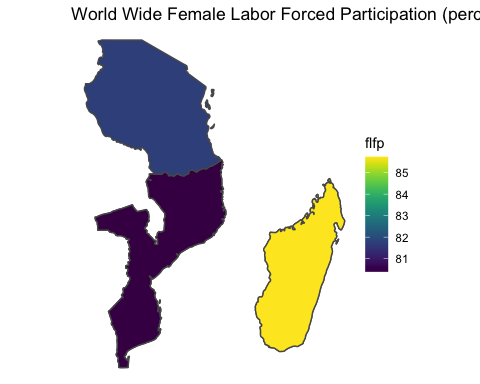
\includegraphics{exam-3_files/figure-latex/unnamed-chunk-7-1.pdf} \#\#
Question 9: In a Shiny app, what are the three main components and their
subcomponents? The app has a user interface object, a server function,
and a call to the shinyApp function.

\hypertarget{question-10-pull-this.pdffile-from-mike-denlys-webpage.-it-is-a-report-that-mike-denly-and-mikefindley-prepared-for-the-us-agency-for-international-development-usaid.}{%
\subsection{Question 10: Pull this.pdffile from Mike Denly's webpage. It
is a report that Mike Denly and MikeFindley prepared for the US Agency
for International Development
(USAID).}\label{question-10-pull-this.pdffile-from-mike-denlys-webpage.-it-is-a-report-that-mike-denly-and-mikefindley-prepared-for-the-us-agency-for-international-development-usaid.}}

\begin{Shaded}
\begin{Highlighting}[]
\CommentTok{\#load libraries}
\FunctionTok{library}\NormalTok{(pdftools)}
\end{Highlighting}
\end{Shaded}

\begin{verbatim}
## Using poppler version 20.12.1
\end{verbatim}

\begin{Shaded}
\begin{Highlighting}[]
\FunctionTok{library}\NormalTok{(tidyr)}
\FunctionTok{library}\NormalTok{(tidytext)}
\FunctionTok{library}\NormalTok{(dplyr)}
\FunctionTok{library}\NormalTok{(stringr)}
\CommentTok{\#retrive pdf}
\NormalTok{armeniatext}\OtherTok{=} \FunctionTok{pdf\_text}\NormalTok{(}\AttributeTok{pdf=}\StringTok{"https://pdf.usaid.gov/pdf\_docs/PA00TNMJ.pdf"}\NormalTok{)}
\end{Highlighting}
\end{Shaded}

\hypertarget{question-11-convert-the-text-pulled-from-this.pdffile-to-a-data-frame-using-the-stringsasfactorsfalse-option.-call-the-data-frame-armeniatext}{%
\subsection{Question 11: Convert the text pulled from this.pdffile to a
data frame, using the, stringsAsFactors=FALSE option. Call the data
frame
armeniatext}\label{question-11-convert-the-text-pulled-from-this.pdffile-to-a-data-frame-using-the-stringsasfactorsfalse-option.-call-the-data-frame-armeniatext}}

\begin{Shaded}
\begin{Highlighting}[]
\CommentTok{\#convert text to data frame}
\NormalTok{armeniatext }\OtherTok{=} \FunctionTok{as.data.frame}\NormalTok{(armeniatext, }\AttributeTok{stringsAsFactors=}\ConstantTok{FALSE}\NormalTok{)}
\NormalTok{armeniatext}\SpecialCharTok{$}\NormalTok{page}\OtherTok{=}\FunctionTok{c}\NormalTok{(}\DecValTok{1}\SpecialCharTok{:}\DecValTok{59}\NormalTok{)}
\FunctionTok{colnames}\NormalTok{(armeniatext)[}\FunctionTok{which}\NormalTok{(}\FunctionTok{names}\NormalTok{(armeniatext)}\SpecialCharTok{==}\StringTok{"armeniatext"}\NormalTok{)] }\OtherTok{\textless{}{-}} \StringTok{"text"}
\end{Highlighting}
\end{Shaded}

\hypertarget{question-12-tokenize-the-data-by-word-and-then-remove-stop-words.}{%
\subsection{Question 12: Tokenize the data by word and then remove stop
words.}\label{question-12-tokenize-the-data-by-word-and-then-remove-stop-words.}}

\begin{Shaded}
\begin{Highlighting}[]
\CommentTok{\#tokenize text and remove stop words}
\NormalTok{armeniatext }\OtherTok{\textless{}{-}}\NormalTok{ armeniatext }\SpecialCharTok{\%\textgreater{}\%} \FunctionTok{unnest\_tokens}\NormalTok{(word, text)}
\FunctionTok{data}\NormalTok{(stop\_words)}
\NormalTok{armeniatext }\OtherTok{\textless{}{-}}\NormalTok{ armeniatext }\SpecialCharTok{\%\textgreater{}\%} \FunctionTok{anti\_join}\NormalTok{(stop\_words)}
\end{Highlighting}
\end{Shaded}

\begin{verbatim}
## Joining, by = "word"
\end{verbatim}

\hypertarget{question-13-figure-out-the-top-5-most-used-word-in-the-report}{%
\subsection{Question 13: Figure out the top 5 most used word in the
report}\label{question-13-figure-out-the-top-5-most-used-word-in-the-report}}

\begin{Shaded}
\begin{Highlighting}[]
\CommentTok{\#count frequency of words}
\NormalTok{hpfreq }\OtherTok{\textless{}{-}}\NormalTok{ armeniatext }\SpecialCharTok{\%\textgreater{}\%} \FunctionTok{count}\NormalTok{(word, }\AttributeTok{sort=} \ConstantTok{TRUE}\NormalTok{)}
\FunctionTok{head}\NormalTok{(hpfreq)}
\end{Highlighting}
\end{Shaded}

\begin{verbatim}
##         word   n
## 1        law 276
## 2 corruption 242
## 3       rule 206
## 4    armenia 195
## 5   european 105
## 6  political 102
\end{verbatim}

\hypertarget{question-14-load-the-billboard-hot-100-webpage-which-we-explored-in-the-course-modules.-namethe-list-objecthot100exam}{%
\subsection{Question 14: Load the Billboard Hot 100 webpage, which we
explored in the course modules. Namethe list
object:hot100exam}\label{question-14-load-the-billboard-hot-100-webpage-which-we-explored-in-the-course-modules.-namethe-list-objecthot100exam}}

\begin{Shaded}
\begin{Highlighting}[]
\CommentTok{\#load libraries}
\FunctionTok{library}\NormalTok{(rvest)}
\end{Highlighting}
\end{Shaded}

\begin{verbatim}
## 
## Attaching package: 'rvest'
\end{verbatim}

\begin{verbatim}
## The following object is masked from 'package:readr':
## 
##     guess_encoding
\end{verbatim}

\begin{Shaded}
\begin{Highlighting}[]
\FunctionTok{library}\NormalTok{(dplyr)}
\FunctionTok{library}\NormalTok{(ggplot2)}
\CommentTok{\#load webpage}
\NormalTok{hot100exam }\OtherTok{\textless{}{-}} \StringTok{"https://www.billboard.com/charts/hot{-}100"}
\NormalTok{hot100 }\OtherTok{\textless{}{-}} \FunctionTok{read\_html}\NormalTok{(hot100exam)}
\end{Highlighting}
\end{Shaded}

\hypertarget{question-use-rvest-to-obtain-identify-all-of-the-nodes-in-the-webpage.}{%
\subsection{Question : Use rvest to obtain identify all of the nodes in
the
webpage.}\label{question-use-rvest-to-obtain-identify-all-of-the-nodes-in-the-webpage.}}

\begin{Shaded}
\begin{Highlighting}[]
\CommentTok{\#declare full (enough) struture to r}
\NormalTok{body\_nodes }\OtherTok{\textless{}{-}}\NormalTok{ hot100 }\SpecialCharTok{\%\textgreater{}\%} 
  \FunctionTok{html\_node}\NormalTok{(}\StringTok{\textquotesingle{}body\textquotesingle{}}\NormalTok{) }\SpecialCharTok{\%\textgreater{}\%} 
  \FunctionTok{html\_children}\NormalTok{()}
\NormalTok{body\_nodes}
\end{Highlighting}
\end{Shaded}

\begin{verbatim}
## {xml_nodeset (37)}
##  [1] <div class="header-wrapper ">\n<header id="site-header" class="site-head ...
##  [2] <div class="site-header__placeholder"></div>
##  [3] <script>\n        var PGM = window.PGM || {};\n        PGM.config = PGM. ...
##  [4] <main id="main" class="page-content"><div id="charts" data-page-title="T ...
##  [5] <div class="ad_desktop dfp-ad dfp-ad-promo " data-position="promo" data- ...
##  [6] <div class="ad-container footerboard footerboard--bottom">\n    <div cla ...
##  [7] <footer id="site-footer" class="site-footer"><div class="container foote ...
##  [8] <div class="biz-modal">\n    <div class="biz-modal__content">\n        < ...
##  [9] <script>\n    window.CLARITY = window.CLARITY || [];\n</script>
## [10] <div class="ad_clarity" data-out-of-page="true" style="display: none;">< ...
## [11] <script>\n\n    window.top.pageLevelKeys = {};\n    window.top.pageAdZon ...
## [12] <script type="text/javascript" async="async" data-cfasync="false" src="h ...
## [13] <script type="text/javascript">\n    let detectDevice = function() {\n   ...
## [14] <script src="https://cdn.cookielaw.org/opt-out/otCCPAiab.js" type="text/ ...
## [15] <script>\n\n    function loadEUScript(source, attributes = {}) {\n\n     ...
## [16] <script src="https://geolocation.onetrust.com/cookieconsentpub/v1/geo/lo ...
## [17] <script src="https://www.billboard.com/assets/1624920239/js/vendors_/art ...
## [18] <script src="https://www.billboard.com/assets/1624920239/js/vendors_/clo ...
## [19] <script src="https://www.billboard.com/assets/1624920239/js/vendors_/rea ...
## [20] <script src="https://www.billboard.com/assets/1624920239/js/vendors_/rea ...
## ...
\end{verbatim}

\begin{Shaded}
\begin{Highlighting}[]
\NormalTok{body\_nodes }\SpecialCharTok{\%\textgreater{}\%} 
  \FunctionTok{html\_children}\NormalTok{()}
\end{Highlighting}
\end{Shaded}

\begin{verbatim}
## {xml_nodeset (9)}
## [1] <header id="site-header" class="site-header " role="banner"><div class="s ...
## [2] <div class="header-wrapper__secondary-header">\n<nav class="site-header-l ...
## [3] <div id="charts" data-page-title="THE HOT 100" data-chart-code="HSI" data ...
## [4] <div class="footerboard-wrapper">\n        <div class="ad_desktop_placeho ...
## [5] <div class="container footer-content">\n\t\t\t\t\t<div class="cover-image ...
## [6] <div class="container">\n\t\t<p class="copyright__paragraph">© 2021 Billb ...
## [7] <div class="container">\n\t\t<p class="station-identification">\n\t\t\tBI ...
## [8] <div class="container">\n\t\t\n\n\n    <div class="ad_desktop dfp-ad dfp- ...
## [9] <div class="biz-modal__content">\n        <button class="biz-modal__close ...
\end{verbatim}

\hypertarget{question-16-use-google-chrome-developer-to-identify-the-necessary-tags-and-pull-the-data-onrankartisttitle-andlast-week.-hint-1-in-class-we-showed-you-how-to-get-the-first-threeof-these.-you-simply-need-to-add-thelast-weekranking.-hint-2-you-can-navigatetwo-ways.-hovering-to-find-what-you-need-or-by-doingcmdf-ctrlfand-usingactual-data-to-find-the-location.-hint-3-youre-looking-to-update-the-code-based-ontheway-the-information-is-in-referenced.-try-out-some-different-options-and-see-whatshows-up-in-the-environment.-keep-trying-until-you-see-that-you-have-achr-1100with-values-that-correspond-to-what-is-in-the-web-page.}{%
\subsection{Question 16: Use Google Chrome developer to identify the
necessary tags and pull the data onRank,Artist,Title, andLast Week. HINT
1: In class we showed you how to get the first threeof these. You simply
need to add theLast Weekranking. HINT 2: You can navigatetwo ways.
Hovering to find what you need or by doingCmd+F / Ctrl+Fand usingactual
data to find the location. HINT 3: You're looking to update the code
based ontheway the information is in referenced. Try out some different
options and see whatshows up in the environment. Keep trying until you
see that you have achr {[}1:100{]}with values that correspond to what is
in the web
page.}\label{question-16-use-google-chrome-developer-to-identify-the-necessary-tags-and-pull-the-data-onrankartisttitle-andlast-week.-hint-1-in-class-we-showed-you-how-to-get-the-first-threeof-these.-you-simply-need-to-add-thelast-weekranking.-hint-2-you-can-navigatetwo-ways.-hovering-to-find-what-you-need-or-by-doingcmdf-ctrlfand-usingactual-data-to-find-the-location.-hint-3-youre-looking-to-update-the-code-based-ontheway-the-information-is-in-referenced.-try-out-some-different-options-and-see-whatshows-up-in-the-environment.-keep-trying-until-you-see-that-you-have-achr-1100with-values-that-correspond-to-what-is-in-the-web-page.}}

\begin{Shaded}
\begin{Highlighting}[]
\CommentTok{\#pull out specific data form the webpage}
\CommentTok{\#rank, artists, title, Last week}
\NormalTok{rank }\OtherTok{\textless{}{-}}\NormalTok{ hot100 }\SpecialCharTok{\%\textgreater{}\%} 
\NormalTok{  rvest}\SpecialCharTok{::}\FunctionTok{html\_nodes}\NormalTok{(}\StringTok{\textquotesingle{}body\textquotesingle{}}\NormalTok{) }\SpecialCharTok{\%\textgreater{}\%} 
\NormalTok{  xml2}\SpecialCharTok{::}\FunctionTok{xml\_find\_all}\NormalTok{(}\StringTok{"//span[contains(@class,}
\StringTok{                     \textquotesingle{}chart{-}element\_\_rank\_\_number\textquotesingle{})]"}\NormalTok{) }\SpecialCharTok{\%\textgreater{}\%} 
\NormalTok{  rvest}\SpecialCharTok{::}\FunctionTok{html\_text}\NormalTok{()}

\NormalTok{artist }\OtherTok{\textless{}{-}}\NormalTok{ hot100 }\SpecialCharTok{\%\textgreater{}\%} 
\NormalTok{  rvest}\SpecialCharTok{::}\FunctionTok{html\_nodes}\NormalTok{(}\StringTok{\textquotesingle{}body\textquotesingle{}}\NormalTok{) }\SpecialCharTok{\%\textgreater{}\%} 
\NormalTok{  xml2}\SpecialCharTok{::}\FunctionTok{xml\_find\_all}\NormalTok{(}\StringTok{"//span[contains(@class,                     \textquotesingle{}chart{-}element\_\_information\_\_artist\textquotesingle{})]"}\NormalTok{) }\SpecialCharTok{\%\textgreater{}\%}
\NormalTok{  rvest}\SpecialCharTok{::}\FunctionTok{html\_text}\NormalTok{()}

\NormalTok{title }\OtherTok{\textless{}{-}}\NormalTok{ hot100 }\SpecialCharTok{\%\textgreater{}\%} 
\NormalTok{  rvest}\SpecialCharTok{::}\FunctionTok{html\_nodes}\NormalTok{(}\StringTok{\textquotesingle{}body\textquotesingle{}}\NormalTok{) }\SpecialCharTok{\%\textgreater{}\%} 
\NormalTok{  xml2}\SpecialCharTok{::}\FunctionTok{xml\_find\_all}\NormalTok{(}\StringTok{"//span[contains(@class,}
\StringTok{ \textquotesingle{}chart{-}element\_\_information\_\_song\textquotesingle{})]"}\NormalTok{) }\SpecialCharTok{\%\textgreater{}\%} 
\NormalTok{  rvest}\SpecialCharTok{::}\FunctionTok{html\_text}\NormalTok{()}

\NormalTok{ last\_week }\OtherTok{\textless{}{-}}\NormalTok{ hot100 }\SpecialCharTok{\%\textgreater{}\%} 
\NormalTok{  rvest}\SpecialCharTok{::}\FunctionTok{html\_nodes}\NormalTok{(}\StringTok{\textquotesingle{}body\textquotesingle{}}\NormalTok{) }\SpecialCharTok{\%\textgreater{}\%} 
\NormalTok{  xml2}\SpecialCharTok{::}\FunctionTok{xml\_find\_all}\NormalTok{(}\StringTok{"//span[contains(@class,}
\StringTok{ \textquotesingle{}chart{-}element\_\_meta text{-}{-}center color{-}{-}secondary text{-}{-}last\textquotesingle{})]"}\NormalTok{) }\SpecialCharTok{\%\textgreater{}\%} 
\NormalTok{  rvest}\SpecialCharTok{::}\FunctionTok{html\_text}\NormalTok{()}
\end{Highlighting}
\end{Shaded}

\hypertarget{question-17-save-all-of-the-files-i.e..rmd.dta.pdfword-doc-push-them-to-your-github-repoand-provide-us-with-the-link-to-that-repo.}{%
\subsection{Question 17: Save all of the files (i.e..Rmd,.dta,.pdf/Word
Doc), push them to your GitHub repo,and provide us with the link to that
repo.}\label{question-17-save-all-of-the-files-i.e..rmd.dta.pdfword-doc-push-them-to-your-github-repoand-provide-us-with-the-link-to-that-repo.}}

\end{document}
